% Options for packages loaded elsewhere
% Options for packages loaded elsewhere
\PassOptionsToPackage{unicode}{hyperref}
\PassOptionsToPackage{hyphens}{url}
\PassOptionsToPackage{dvipsnames,svgnames,x11names}{xcolor}
%
\documentclass[
  letterpaper,
  DIV=11,
  numbers=noendperiod]{scrartcl}
\usepackage{xcolor}
\usepackage{amsmath,amssymb}
\setcounter{secnumdepth}{-\maxdimen} % remove section numbering
\usepackage{iftex}
\ifPDFTeX
  \usepackage[T1]{fontenc}
  \usepackage[utf8]{inputenc}
  \usepackage{textcomp} % provide euro and other symbols
\else % if luatex or xetex
  \usepackage{unicode-math} % this also loads fontspec
  \defaultfontfeatures{Scale=MatchLowercase}
  \defaultfontfeatures[\rmfamily]{Ligatures=TeX,Scale=1}
\fi
\usepackage{lmodern}
\ifPDFTeX\else
  % xetex/luatex font selection
\fi
% Use upquote if available, for straight quotes in verbatim environments
\IfFileExists{upquote.sty}{\usepackage{upquote}}{}
\IfFileExists{microtype.sty}{% use microtype if available
  \usepackage[]{microtype}
  \UseMicrotypeSet[protrusion]{basicmath} % disable protrusion for tt fonts
}{}
\makeatletter
\@ifundefined{KOMAClassName}{% if non-KOMA class
  \IfFileExists{parskip.sty}{%
    \usepackage{parskip}
  }{% else
    \setlength{\parindent}{0pt}
    \setlength{\parskip}{6pt plus 2pt minus 1pt}}
}{% if KOMA class
  \KOMAoptions{parskip=half}}
\makeatother
% Make \paragraph and \subparagraph free-standing
\makeatletter
\ifx\paragraph\undefined\else
  \let\oldparagraph\paragraph
  \renewcommand{\paragraph}{
    \@ifstar
      \xxxParagraphStar
      \xxxParagraphNoStar
  }
  \newcommand{\xxxParagraphStar}[1]{\oldparagraph*{#1}\mbox{}}
  \newcommand{\xxxParagraphNoStar}[1]{\oldparagraph{#1}\mbox{}}
\fi
\ifx\subparagraph\undefined\else
  \let\oldsubparagraph\subparagraph
  \renewcommand{\subparagraph}{
    \@ifstar
      \xxxSubParagraphStar
      \xxxSubParagraphNoStar
  }
  \newcommand{\xxxSubParagraphStar}[1]{\oldsubparagraph*{#1}\mbox{}}
  \newcommand{\xxxSubParagraphNoStar}[1]{\oldsubparagraph{#1}\mbox{}}
\fi
\makeatother


\usepackage{longtable,booktabs,array}
\usepackage{calc} % for calculating minipage widths
% Correct order of tables after \paragraph or \subparagraph
\usepackage{etoolbox}
\makeatletter
\patchcmd\longtable{\par}{\if@noskipsec\mbox{}\fi\par}{}{}
\makeatother
% Allow footnotes in longtable head/foot
\IfFileExists{footnotehyper.sty}{\usepackage{footnotehyper}}{\usepackage{footnote}}
\makesavenoteenv{longtable}
\usepackage{graphicx}
\makeatletter
\newsavebox\pandoc@box
\newcommand*\pandocbounded[1]{% scales image to fit in text height/width
  \sbox\pandoc@box{#1}%
  \Gscale@div\@tempa{\textheight}{\dimexpr\ht\pandoc@box+\dp\pandoc@box\relax}%
  \Gscale@div\@tempb{\linewidth}{\wd\pandoc@box}%
  \ifdim\@tempb\p@<\@tempa\p@\let\@tempa\@tempb\fi% select the smaller of both
  \ifdim\@tempa\p@<\p@\scalebox{\@tempa}{\usebox\pandoc@box}%
  \else\usebox{\pandoc@box}%
  \fi%
}
% Set default figure placement to htbp
\def\fps@figure{htbp}
\makeatother


% definitions for citeproc citations
\NewDocumentCommand\citeproctext{}{}
\NewDocumentCommand\citeproc{mm}{%
  \begingroup\def\citeproctext{#2}\cite{#1}\endgroup}
\makeatletter
 % allow citations to break across lines
 \let\@cite@ofmt\@firstofone
 % avoid brackets around text for \cite:
 \def\@biblabel#1{}
 \def\@cite#1#2{{#1\if@tempswa , #2\fi}}
\makeatother
\newlength{\cslhangindent}
\setlength{\cslhangindent}{1.5em}
\newlength{\csllabelwidth}
\setlength{\csllabelwidth}{3em}
\newenvironment{CSLReferences}[2] % #1 hanging-indent, #2 entry-spacing
 {\begin{list}{}{%
  \setlength{\itemindent}{0pt}
  \setlength{\leftmargin}{0pt}
  \setlength{\parsep}{0pt}
  % turn on hanging indent if param 1 is 1
  \ifodd #1
   \setlength{\leftmargin}{\cslhangindent}
   \setlength{\itemindent}{-1\cslhangindent}
  \fi
  % set entry spacing
  \setlength{\itemsep}{#2\baselineskip}}}
 {\end{list}}
\usepackage{calc}
\newcommand{\CSLBlock}[1]{\hfill\break\parbox[t]{\linewidth}{\strut\ignorespaces#1\strut}}
\newcommand{\CSLLeftMargin}[1]{\parbox[t]{\csllabelwidth}{\strut#1\strut}}
\newcommand{\CSLRightInline}[1]{\parbox[t]{\linewidth - \csllabelwidth}{\strut#1\strut}}
\newcommand{\CSLIndent}[1]{\hspace{\cslhangindent}#1}



\setlength{\emergencystretch}{3em} % prevent overfull lines

\providecommand{\tightlist}{%
  \setlength{\itemsep}{0pt}\setlength{\parskip}{0pt}}



 


\KOMAoption{captions}{tableheading}
\makeatletter
\@ifpackageloaded{caption}{}{\usepackage{caption}}
\AtBeginDocument{%
\ifdefined\contentsname
  \renewcommand*\contentsname{Table of contents}
\else
  \newcommand\contentsname{Table of contents}
\fi
\ifdefined\listfigurename
  \renewcommand*\listfigurename{List of Figures}
\else
  \newcommand\listfigurename{List of Figures}
\fi
\ifdefined\listtablename
  \renewcommand*\listtablename{List of Tables}
\else
  \newcommand\listtablename{List of Tables}
\fi
\ifdefined\figurename
  \renewcommand*\figurename{Figure}
\else
  \newcommand\figurename{Figure}
\fi
\ifdefined\tablename
  \renewcommand*\tablename{Table}
\else
  \newcommand\tablename{Table}
\fi
}
\@ifpackageloaded{float}{}{\usepackage{float}}
\floatstyle{ruled}
\@ifundefined{c@chapter}{\newfloat{codelisting}{h}{lop}}{\newfloat{codelisting}{h}{lop}[chapter]}
\floatname{codelisting}{Listing}
\newcommand*\listoflistings{\listof{codelisting}{List of Listings}}
\makeatother
\makeatletter
\makeatother
\makeatletter
\@ifpackageloaded{caption}{}{\usepackage{caption}}
\@ifpackageloaded{subcaption}{}{\usepackage{subcaption}}
\makeatother
\usepackage{bookmark}
\IfFileExists{xurl.sty}{\usepackage{xurl}}{} % add URL line breaks if available
\urlstyle{same}
\hypersetup{
  pdftitle={Childcare Costs \& Female Labor Force Participation},
  colorlinks=true,
  linkcolor={blue},
  filecolor={Maroon},
  citecolor={Blue},
  urlcolor={Blue},
  pdfcreator={LaTeX via pandoc}}


\title{Childcare Costs \& Female Labor Force Participation}
\usepackage{etoolbox}
\makeatletter
\providecommand{\subtitle}[1]{% add subtitle to \maketitle
  \apptocmd{\@title}{\par {\large #1 \par}}{}{}
}
\makeatother
\subtitle{DSAN 5650: Causal Inference for Computational Social Science}
\author{Emily Mitchum}
\date{2026-08-10}
\begin{document}
\maketitle
\begin{abstract}
A substantial body of research has found that reductions in childcare
costs are positively associated with increased maternal labor-force
participation. However, when analyzing the elasticity of employment to
childcare prices, researchers find heterogeneity across various
geographies and time-periods. This may be attributable to differences in
educational attainment, labor force attachment, and other factors (.
This research paper uses U.S. county-level data to examine whether the
association between childcare affordability and maternal labor-force
participation among women with children under age six varies across
local occupational contexts. I present a Bayesian logit-normal
regression model that estimates maternal labor force participation as a
function of childcare affordability, the county share of workers in
``greedy'' occupations, educational attainment, geographic rootedness,
and an interaction between childcare burden and occupational structure.
Aligning with existing research, I find that higher childcare burden is
associated with lower maternal labor force participation. However, I
also find that this negative association becomes weaker as a county's
concentration of women in greedy occupations increases. Educational
attainment and geographic rootedness are also moderately associated with
maternal labor force participation, while greedy-occupation-share is
weakly associated.
\end{abstract}


\subsection{Introduction}\label{sec-1}

Earlier this year, I examined the major factors that help explain U.S.
maternal labor force participation trends and persistent wage
differentials between men and women. Existing research consistently
identifies motherhood as an important contributor to both reduced
labor-force participation and long-term earnings penalties.

Childcare costs, which have significantly outpaced overall inflation,
play a significant role in women's ability or decision to remain in the
workforce. This trend has driven an overall focus within the research
community on the relationship between childcare affordability and
maternal labor force participation. Research has appropriately paid
particular attention to low-income women, for whom childcare expenses
represent a large share of potential earnings, and whose labor market
attachment is the most impacted by childcare costs (Havnes and Mogstad
(2011)).

Several studies have concluded that reducing childcare costs would
increase maternal employment, especially among low-income women. The
majority of U.S. childcare assistance programs are also primarily
available for lower-income households and reach only a minority of
eligible families. Less is known about this association amongst women in
moderate or high income brackets, who remain burdened by high childcare
costs. For these women, childcare constraints may impact labor force
participation differently. Increased earning potential and financial
resources may make them more likely to remain employed despite high
childcare costs, while reducing hours or seeking work flexibility to
meet childcare demands. This behavior may ultimately result in reduced
career advancement and lower wages.

This paper tests this theory, using county-level data to analyze how
women in different occupational contexts may respond differently to
childcare costs. I use the concentration of women working in ``greedy''
occupations, or high-paying occupations that disproportionately reward
long hours and constant availability, to measure local occupational
context. This is used to test whether the known association between
childcare burden and maternal labor-force participation is moderated by
occupation ``greediness''.

County-level female labor force participation only determines whether
mothers participate in the labor force, rather than how many hours they
work. Therefore, this analysis does not directly model the wage gap.
However, beginning to understand potential effect heterogeneity in this
relationship may help explain persistent gender gaps in earnings despite
comparable levels of overall labor-force participation.

\subsection{Background and Conceptual
Framework}\label{background-and-conceptual-framework}

\subsubsection{Existing Childcare Policy and Maternal
Employment}\label{existing-childcare-policy-and-maternal-employment}

Researchers generally agree that increased investment in childcare
affordability interventions results in higher maternal labor force
participation, particularly among low-income women in the first few
years after birth. For instance, Burgess, Chien and Enchautegui find
that increasing Child Care and Development Block Grant (CCDBG)
expenditures by 10-percent per child would increase employment levels
among low-income women with young children by between half to two-thirds
of a percent ({``The {Effects} of {Child} {Care} {Subsidies} on
{Maternal} {Labor} {Force} {Participation} in the {United} {States}''}
(2016)).

Still, the majority of U.S. childcare assistance programs reach only a
subset of families and are concentrated among lower-income households.
The Child Care and Development Block Grant (CCDBG) is only available for
families who make less than 85\% of their state median income. Even
amongst those that meet requirements, federal childcare subsidies only
reach approximately 14\% of eligible families ({``Factsheet: {Estimates}
of {Child} {Care} {Eligibility} and {Receipt} for {Fiscal} {Year}
2017''} (2020)), and state subsidies reach only approximately 22\% of
eligible families. Tax incentives, including the Child and Dependent
Care Tax Credit, also benefit a minority of families with children due
to its non-refundable structure, steep income phase-downs, and
restrictions that require two working parents. (Araujo, McBride, and
Sandler (2025))

While most childcare programs focus on low-income families, evidence
from universal early childcare programs suggests that reducing childcare
constraints can affect maternal employment across a broader range of
women. Two years after implementing a universal pre-kindergarten program
in 2008, D.C. observed a 12\% increase in the maternal labor force
participation rate. A study from the Center for American Progress found
that this increase was strongly associated with implementation of
universal preschool (Malik, Rasheed (2018)). This example is
particularly important given D.C.'s occupational profile, with an
unusually large concentration of highly-educated women in high-paying,
senior positions. This example motivates the current analysis, which
seeks to understand the varying slope of the relationship between
childcare affordability and labor force participation among counties
with different female occupational profiles.

\subsubsection{Occupational
``Greediness''}\label{occupational-greediness}

This analysis builds on existing research from economist Claudia Goldin,
who has extensively studied ``greedy occupations''. Goldin finds that
greedy occupations lead women to remain employed, even as they have
children, but earn less over time, due to childcare responsibilities
that prevent them from meeting demanding work requirements, including
long hours and travel (Goldin (2014)). Women's role as primary
care-givers leads them to take career breaks, reduce hours, and trade
high-stress roles for flexible roles.

Goldin identifies finance, law, consulting, and corporate management as
common greedy occupations, characterized by time inflexibility, low work
substitutability, and non-linear pay. These occupations drive gender pay
differentials, since women are more likely to experience childcare
related work interruptions and less likely to be able to work rigid
schedules (Sobeck (2024)). Using Goldin's research as a framework, I
model county-level occupational greediness by sex using U.S. Census
adult employment statistics.

\subsubsection{Educational Attainment}\label{educational-attainment}

Educational attainment is closely related to occupation context and
labor force participation. Geographies with a greater share of
individuals with advanced degrees are more likely to have higher
concentrations of individuals in advanced white-collar occupations.
Women in these occupations are more likely to have greater earning
power, which also influences their labor force attachment. I model
educational attainment as the share of individuals in each county with
at least a bachelor's degree. This is used to determine if the effect of
greedy occupation structure is partially or completely explained by
county educational composition.

\subsubsection{Geographic ``Rootedness'' and Informal Childcare
Support}\label{geographic-rootedness-and-informal-childcare-support}

Informal childcare support, through family-members, friends and
neighbors, can provide mothers with relief from exorbitant childcare
costs, as well as unmatched flexibility. However, the availability of
local support varies across households. Highly-educated and high-income
individuals are often more likely to move away from their birthplace,
where family resides, to regions with greater economic opportunities for
higher-paying jobs. While over half of U.S. adults report living within
an hour of family, a Pew Research study found that upper-income adults
and adults with a postgraduate degree were the most likely to report
living near no extended family (Hurst (2022)).

Existing literature suggests that access to informal familial childcare
can influence maternal labor force participation. Compton and Pollak
find that married women with young children that live within close
proximity of mothers or mothers-in-law are predicted to have a 4 to 10
percent higher labor force participation rate when compared to women
that live farther from family (Compton and Pollak (2014)). They theorize
that family members within close proximity provide ``insurance'' to
working mothers, by being available to provide care in irregular or
unanticipated circumstances. Building upon this framework, I use
geographic rootedness as a proxy for access to local familial childcare.
I model geographic ``rootedness'' as the share of adults 25 or older in
each county who report living in the state they were born in. While this
does not directly estimate the proximity of family or availability of
informal childcare, it provides a county-level profile of geographic
attachment to measure potential differences in access to informal
childcare support.

\subsection{Data and Measures}\label{data-and-measures}

\subsubsection{Data Sources}\label{data-sources}

This analysis uses 2022 data from the Department of Labor's National
Database of Childcare Prices (NDCP) to retrieve each county's maternal
female labor force participation rate (FLPR) for women with children
under 6, the outcome variable, and childcare costs, which are used to
determine the childcare cost burden. The American Community Survey (ACS)
five-year estimates are used to identify the median family income, share
of bachelor's-plus individuals, female greedy occupation share, and
geographic rootedness. This county level data is merged using
FIPS-codes, resulting in a final sample of 2,653 counties. 491 counties
are excluded from the sample as a result of missing any of the modeled
variables. Exclusion is primarily a result of missing childcare data,
including complete state absences in Pennsylvania, Indiana, Vermont, and
New Mexico, due to low response rates or too few childcare providers.
This is a known limitation of the NDCP.

\subsubsection{Data Transformations}\label{data-transformations}

FLPR is first converted from a percentage to a proportion. Exact 0 and 1
FLPR values are then slightly adjusted, since the logit function is
undefined at those exact values. Greedy occupation share is represented
by the proportion of eligible employed women working in greedy
occupations. Bachelor's-plus share is calculated as the proportion of
adults age 25 and older with at least a bachelor's degree. Finally,
geographic rootedness is calculated as the proportion of adults age 25
and older who were born in their current state of residence. All
continuous predictors are standardized to have mean zero and standard
deviation prior to modeling.

\subsubsection{Data and Measures
Summary}\label{data-and-measures-summary}

The sources and representations of each variable are summarized below:

\begin{longtable}[]{@{}
  >{\raggedright\arraybackslash}p{(\linewidth - 4\tabcolsep) * \real{0.3333}}
  >{\raggedright\arraybackslash}p{(\linewidth - 4\tabcolsep) * \real{0.3333}}
  >{\raggedright\arraybackslash}p{(\linewidth - 4\tabcolsep) * \real{0.3333}}@{}}
\caption{Data Sources and Variable
Representations}\label{tbl-0}\tabularnewline
\toprule\noalign{}
\begin{minipage}[b]{\linewidth}\raggedright
Variable
\end{minipage} & \begin{minipage}[b]{\linewidth}\raggedright
Source(s)
\end{minipage} & \begin{minipage}[b]{\linewidth}\raggedright
Representation
\end{minipage} \\
\midrule\noalign{}
\endfirsthead
\toprule\noalign{}
\begin{minipage}[b]{\linewidth}\raggedright
Variable
\end{minipage} & \begin{minipage}[b]{\linewidth}\raggedright
Source(s)
\end{minipage} & \begin{minipage}[b]{\linewidth}\raggedright
Representation
\end{minipage} \\
\midrule\noalign{}
\endhead
\bottomrule\noalign{}
\endlastfoot
Maternal Female Labor Force Participation Rate (FLPR) & Department of
Labor (DOL) county data & Labor-force participation rate among women
with children under age six \\
Childcare cost burden & DOL National Database of Childcare Prices;
American Community Survey (ACS) median family income & Annual
center-based childcare cost for children ages 0--5 divided by median
family income \\
Greedy occupation share & ACS Occupation by Sex for the Civilian
Employed Population 16 Years and Over (Series S240) & Share of employed
women in management, business and financial, and legal occupations \\
Educational attainment & ACS Place of Birth by Educational Attainment in
the United States (Series B06009) & Share of adults age 25 or older with
a bachelor's, graduate, or professional degree \\
Geographic rootedness & ACS Place of Birth by Educational Attainment in
the United States (Series B06009) & Share of adults age 25 or older who
were born in their current state of residence \\
\end{longtable}

\subsection{Empirical Strategy}\label{empirical-strategy}

\subsubsection{Naive Model: FLPR as a Function of Childcare
Burden}\label{naive-model-flpr-as-a-function-of-childcare-burden}

First, I analyze a naive logit-Normal regression model of female labor
force participation as a function of only childcare burden.

This relationship can be written as:
\begin{equation}\phantomsection\label{eq-1}{
y_i = \beta_0 + \beta_{C}c_i
}\end{equation}

where \(i\) indexes counties, \(y_i\) is the female labor force
participation rate, \(\beta_0\) represents the baseline female labor
force participation rate when childcare burden is held constant, or at
an average childcare burden across counties, and \(\beta_C\) represents
the strength of the relationship between childcare cost burden and
female labor force participation.

County-level FLPR resembles a normal distribution, therefore, FLPR is
modeled using a normal likelihood. The intercept term, or baseline
female labor force participation rate, is drawn from a normal
distribution with a prior mean of 0.847, or
\(\(\operatorname{logit}(0.70)\)\), with \(\sigma=.25\) to allow for
some uncertainty. This rate is close to the empirical FLPR mean of 70\%
across counties. Childcare burden is modeled with a weakly informative
prior of \(\mu=0, \sigma=0.15\), assuming no direction of relationship,
but expecting few extreme values.

Figure 1 shows a Bayesian probabilistic graphical model (PGM) depicting
the Naive model.

\pandocbounded{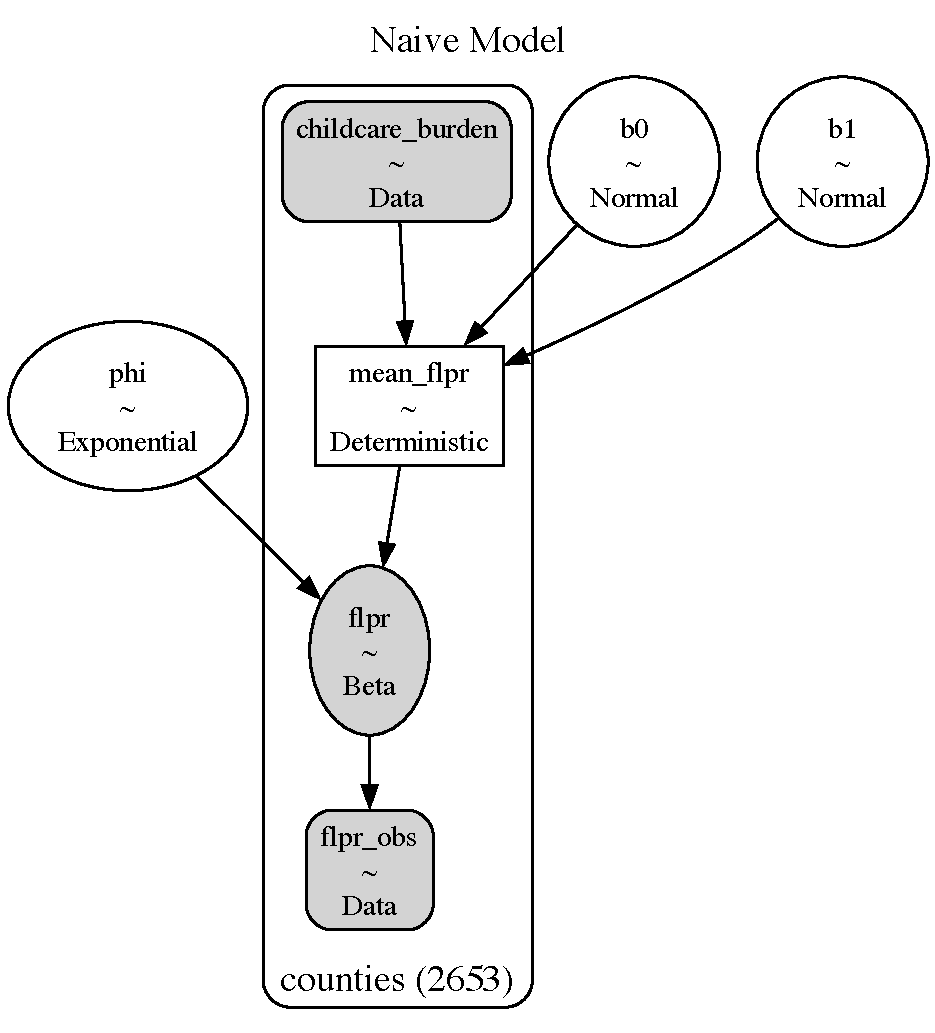
\includegraphics[keepaspectratio]{index_files/mediabag/assets/naive_model.pdf}}

\subsubsection{Adjusting for Covariates}\label{adjusting-for-covariates}

Next, I fit progressively more complex models, adding relevant
covariates and comparing coefficient estimates. All models are estimated
using Bayesian logit-Normal regression. This approach allows me to
assess robustness of the estimated relationships after adjusting for
educational attainment and geographic rootedness and whether these
variables account for part of the association attributed to greedy
occupational structure. Like childcare burden, all covariates are
modeled with weakly informative priors of \(\mu=0, \sigma=0.15\).

\subsubsection{Hypotheses}\label{hypotheses}

My predictions about the relationships between county-level childcare
cost burden, greedy occupation share, educational attainment, and
geographic rootedness yield the following hypotheses:

\begin{itemize}
\tightlist
\item
  \textbf{Hypothesis 1.} \(\beta_{C} < 0\) (\emph{hypothesized causal
  mechanism}: higher childcare cost burden is associated with lower
  county-level maternal labor-force participation).
\item
  \textbf{Hypothesis 2.} \(\beta_{CG} > 0\) (\emph{hypothesized causal
  mechanism}: the negative association between childcare burden and
  maternal labor-force participation weakens as greedy occupation share
  increases).
\item
  \textbf{Hypothesis 3.} \(\beta_{B} > 0\) (\emph{hypothesized causal
  mechanism}: inclusion of educational attainment reduces the estimated
  coefficient of greedy occupation share, indicating that educational
  composition accounts for part of the initially observed association).
\item
  \textbf{Hypothesis 4.} \(\beta_{R} > 0\) (\emph{hypothesized causal
  mechanism}: county-level geographic rootedness is associated with
  higher maternal labor-force participation, potentially because
  rootedness is associated with stronger access to informal family
  support networks).
\end{itemize}

\subsubsection{``Greedy'' Model}\label{greedy-model}

The next model, the ``greedy'' model, introduces county occupation
greediness and its interaction with childcare burden.

This relationship can be written as:

\[
yi = \beta_0 + \beta_{C}ci + \beta_{G}gi + \beta_{CG}cgi
\]

where \(\beta_G\) represents the association between greedy occupation
share and maternal FLPR while holding childcare burden constant, and
\(\beta_{CG}\) represents an interaction between childcare burden and
greedy occupation share. \(\beta_{CG}\) is used to measure whether the
relationship between childcare burden and FLPR varies across
occupational contexts.

To ease interpretation of \(\beta_{CG}\), I later estimate the change in
predicted FLPR associated with moving from average childcare burden to
one standard deviation above average at low, average, and high levels of
greedy occupation share.

\subsubsection{Education-Adjusted Model}\label{education-adjusted-model}

The education-adjusted model introduces the share of county residents
with a bachelor's degree or greater advanced degree.

This relationship can be written as:

\[
yi = \beta_0 + \beta_{C}ci + \beta_{G}gi + \beta_{CG}cgi + \beta_{B}bi
\]

where \(\beta_{B}\) represents the association between educational
attainment and maternal FLPR while holding other variables constant.
This is used to test whether occupation context is partially or
completely explained by education attainment. The greedy-occupation
coefficient across Models 2 and 3 are thus compared to assess changes in
direction or magnitude after education is included.

\subsubsection{Fully Adjusted ``Rooted''
Model}\label{fully-adjusted-rooted-model}

The final fully adjusted model, or ``rooted'' model, introduces
geographical rootedness, measured as the share of adults age 25 and
older who were born in their current state of residence.

This relationship can be written as:

\[
yi = \beta_0 + \beta_{C}ci + \beta_{G}gi + \beta_{CG}cgi + \beta_{B}bi + \beta_{R}ri
\]

where \(\beta_{R}\) represents the association between geographical
rootness and maternal FLPR while holding other variables constant.
Rootedness is included as a proxy for access to informal familial
childcare and used to test whether differing geographic attachment
profiles between counties are partially responsible for the other
estimated relationships.

\subsection{Results}\label{sec-4}

\subsubsection{Poseterior Estimates}\label{poseterior-estimates}

The following table shows posterior estimates for each model
specification. Within each cell, the first value is the posterior mean,
and the second is the 89\% credible interval, shown within brackets. All
values are shown on the logit scale.

\begin{longtable}[]{@{}
  >{\raggedright\arraybackslash}p{(\linewidth - 8\tabcolsep) * \real{0.2000}}
  >{\raggedleft\arraybackslash}p{(\linewidth - 8\tabcolsep) * \real{0.2000}}
  >{\raggedleft\arraybackslash}p{(\linewidth - 8\tabcolsep) * \real{0.2000}}
  >{\raggedleft\arraybackslash}p{(\linewidth - 8\tabcolsep) * \real{0.2000}}
  >{\raggedleft\arraybackslash}p{(\linewidth - 8\tabcolsep) * \real{0.2000}}@{}}
\caption{Posterior estimates of model
specifications}\label{tbl-1}\tabularnewline
\toprule\noalign{}
\begin{minipage}[b]{\linewidth}\raggedright
Parameter
\end{minipage} & \begin{minipage}[b]{\linewidth}\raggedleft
Naive
\end{minipage} & \begin{minipage}[b]{\linewidth}\raggedleft
Greedy
\end{minipage} & \begin{minipage}[b]{\linewidth}\raggedleft
+ Education
\end{minipage} & \begin{minipage}[b]{\linewidth}\raggedleft
+ Rootedness
\end{minipage} \\
\midrule\noalign{}
\endfirsthead
\toprule\noalign{}
\begin{minipage}[b]{\linewidth}\raggedright
Parameter
\end{minipage} & \begin{minipage}[b]{\linewidth}\raggedleft
Naive
\end{minipage} & \begin{minipage}[b]{\linewidth}\raggedleft
Greedy
\end{minipage} & \begin{minipage}[b]{\linewidth}\raggedleft
+ Education
\end{minipage} & \begin{minipage}[b]{\linewidth}\raggedleft
+ Rootedness
\end{minipage} \\
\midrule\noalign{}
\endhead
\bottomrule\noalign{}
\endlastfoot
\(\beta_{0}\) (Intercept) & 1.172 {[}1.10, 1.20{]} & 1.167 {[}1.10,
1.20{]} & 1.167 {[}1.10, 1.20{]} & 1.168 {[}1.10, 1.20{]} \\
\(\beta_{c}\) (Childcare burden) & -0.107 {[}-0.160, -0.058{]} & -0.120
{[}-0.170, -0.070{]} & -0.122 {[}-0.170, -0.076{]} & -0.103 {[}-0.150,
-0.052{]} \\
\(\beta_{G}\) (Greedy occupation share) & --- & 0.112 {[}0.064, 0.160{]}
& 0.067 {[}0.010, 0.130{]} & 0.085 {[}0.026, 0.140{]} \\
\(\beta_{CG}\) (Childcare burden × greedy share) & --- & 0.072 {[}0.026,
0.120{]} & 0.069 {[}0.022, 0.120{]} & 0.070 {[}0.023, 0.110{]} \\
\(\beta_{B}\) (Bachelor's-plus attainment) & --- & --- & 0.084 {[}0.024,
0.140{]} & 0.155 {[}0.092, 0.220{]} \\
\(\beta_{R}\) (Born-in-state share) & --- & --- & --- & 0.173 {[}0.120,
0.230{]} \\
\end{longtable}

\(\beta_{C}\), representing the childcare burden estimate, remains
relatively stable across models. Notably, the interaction term,
\(\beta_{CG}\), is very stable, which suggests that inclusion of
educational attainment and geographic rootedness does not eliminate
heterogeneity. Inclusion of educational attainment significantly reduces
the strength of \(\beta_{G}\), greedy occupation share, from 0.112 to
0.067. This suggests that differences in educational attainment between
counties account for a large part of the earlier observed association
between occupational greediness and FLPR. However, once geographical
rootedness, \(\beta_{R}\), is included, occupational greediness's
coefficient increases to 0.085. This suggests that the relationships
among these three variables are partially overlapping.

\subsubsection{Heterogeneity in the Estimated Association between
Childcare Burden and
FLPR}\label{heterogeneity-in-the-estimated-association-between-childcare-burden-and-flpr}

Using the fully adjusted model, we now examine the predicted FLPR
associated with moving from average childcare burden to one standard
deviation above average at low, average, and high levels of greedy
occupation share. The following table and figure show clearly different
slopes of the relationship between childcare burden and FLPR across
occupational contexts.

\pandocbounded{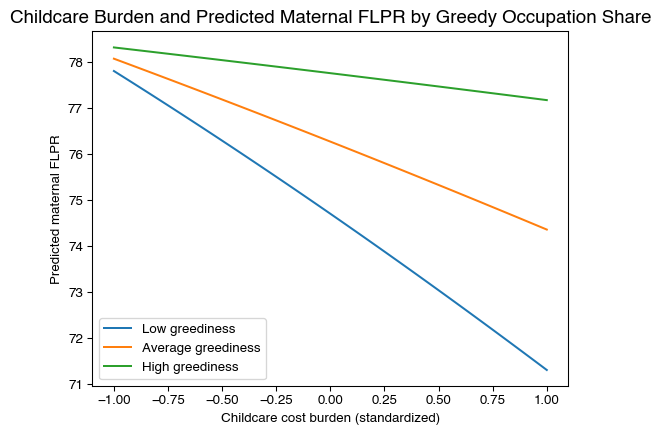
\includegraphics[keepaspectratio]{assets/heterogeneity_plot.png}}

\begin{longtable}[]{@{}
  >{\raggedright\arraybackslash}p{(\linewidth - 6\tabcolsep) * \real{0.2500}}
  >{\raggedleft\arraybackslash}p{(\linewidth - 6\tabcolsep) * \real{0.2500}}
  >{\raggedleft\arraybackslash}p{(\linewidth - 6\tabcolsep) * \real{0.2500}}
  >{\raggedleft\arraybackslash}p{(\linewidth - 6\tabcolsep) * \real{0.2500}}@{}}
\caption{Posterior estimated change in maternal FLPR associated with an
increase in childcare burden from the sample mean to one SD above the
mean, evaluated at low, average, and high levels of occupational
greediness.}\label{tbl-2}\tabularnewline
\toprule\noalign{}
\begin{minipage}[b]{\linewidth}\raggedright
Occupational Profile
\end{minipage} & \begin{minipage}[b]{\linewidth}\raggedleft
Mean change in FLPR
\end{minipage} & \begin{minipage}[b]{\linewidth}\raggedleft
SD
\end{minipage} & \begin{minipage}[b]{\linewidth}\raggedleft
89\% credible interval
\end{minipage} \\
\midrule\noalign{}
\endfirsthead
\toprule\noalign{}
\begin{minipage}[b]{\linewidth}\raggedright
Occupational Profile
\end{minipage} & \begin{minipage}[b]{\linewidth}\raggedleft
Mean change in FLPR
\end{minipage} & \begin{minipage}[b]{\linewidth}\raggedleft
SD
\end{minipage} & \begin{minipage}[b]{\linewidth}\raggedleft
89\% credible interval
\end{minipage} \\
\midrule\noalign{}
\endhead
\bottomrule\noalign{}
\endlastfoot
Low greedy (-1 SD) & -3.40 & 0.92 & {[}-4.90, -1.90{]} \\
Average greedy (0 SD) & -1.91 & 0.60 & {[}-2.90, -0.96{]} \\
High greedy (+1 SD) & -0.59 & 0.72 & {[}-1.70, 0.55{]} \\
\end{longtable}

Aligning with existing research, counties with low levels of
occupational greediness, shown by the blue line, show the steepest
slope. This suggests that maternal FLPR is the most sensitive to
childcare cost burden in these counties. Notably, the strength of the
association begins to weaken when analyzing counties with average
ocucpational greediness, shown in orange, and appears nearly flat when
analyzing counties with high occupational greediness, shown in green.

\subsection{Discussion}\label{discussion}

These results align with existing research, suggesting that higher
childcare burden is associated with lower maternal labor force
participation. They also expand existing analysis of the naive
association between childcare cost burden and maternal FLPR by showing
that this relationship varies across county occupational contexts. The
well-established negative association between childcare burden and
maternal FLPR is highest amongst counties with a relatively low share of
women in greedy occupations and weakens significantly as greedy
occupation share increases.

This observed occupational hetereogenity aligns with the intuition that
women in communities with high concentrations of high-earning,
prestigious professions may be less likely to leave the labor force when
responding to increases in childcare costs. However, because this model
uses county-level estimates, it should not be interpreted to mean that
individual women employed in greedy occupations are responsible for this
effect heterogenity.

Including bachelor's plus share weakens the observed association between
occupational greediness and maternal FLPR, indicating that county level
differences in educational attainment partially account for this
association. However, it notably does not reduce the effect of the
interaction between childcare burden and occupation greediness. The
model results also showed a positive association between Geographic
rootedness and maternal FLPR. Interestingly, the strength of this
association was even larger than educational attainment, a well-known
factor strongly associated with FLPR. If geographic rootedness provides
a fair proxy of familial childcare availability, this suggests that
access to such support reduces childare constraints, allowing mothers to
remain in the workforce. However, it is important to note that while the
estimated associations between variables remain relatively consistent
across models, each model only explains a small amount of variation in
maternal FLPR between counties.

\subsection{Conclusions}\label{conclusions}

This paper strengthens existing research by affirming that childcare
burden is negatively associated with female labor force participation.
It builds upon the current body of knowledge by uncovering that this
association is partially moderated by local occupational contexts.
Results also indicate that acces to familial support networks may also
shape the slope of the relationship between female labor force
participation and childcare costs. It also highlights a need for
additional research, as both the naive model of maternal FLPR as a
function solely of childcare and the fully adjusted model explain only a
small amount of variation in maternal FLPR between counties. Ultimatley,
this analysis offerse important context to researchers and
policy-makers, by providing insight into why estimated employment
responses to childcare affordability interventions vary.

\subsection{References}\label{references}

\phantomsection\label{refs}
\begin{CSLReferences}{1}{0}
\bibitem[\citeproctext]{ref-araujo_impact_2025}
Araujo, Valeska, Linden McBride, and Danielle H Sandler. 2025. {``The
{Impact} of {Childcare} {Costs} on {Mothers}' {Labor} {Force}
{Participation},''} April.

\bibitem[\citeproctext]{ref-bureau_american_nodate}
Bureau, US Census. n.d.
{``\href{https://www.census.gov/data/developers/data-sets/acs-5year.html}{American
{Community} {Survey} 5-{Year} {Data} (2009-2024)}.''} \emph{Census.gov}.
Accessed August 8, 2026.

\bibitem[\citeproctext]{ref-compton_family_2014}
Compton, Janice, and Robert A. Pollak. 2014.
{``\href{https://doi.org/10.1016/j.jue.2013.03.007}{Family Proximity,
Childcare, and Women's Labor Force Attachment}.''} \emph{Journal of
Urban Economics}, Spatial {Dimensions} of {Labor} {Markets}, 79
(January): 72--90.

\bibitem[\citeproctext]{ref-noauthor_factsheet_2020}
{``\href{http://aspe.hhs.gov/reports/factsheet-estimates-child-care-eligibility-receipt-fiscal-year-2017}{Factsheet:
{Estimates} of {Child} {Care} {Eligibility} and {Receipt} for {Fiscal}
{Year} 2017}.''} 2020. \emph{ASPE}.

\bibitem[\citeproctext]{ref-goldin_grand_2014}
Goldin, Claudia. 2014.
{``\href{https://doi.org/10.1257/aer.104.4.1091}{A {Grand} {Gender}
{Convergence}: {Its} {Last} {Chapter}}.''} \emph{American Economic
Review} 104 (4): 1091--1119.

\bibitem[\citeproctext]{ref-havnes_no_2011}
Havnes, Tarjei, and Magne Mogstad. 2011.
{``\href{https://www.jstor.org/stable/41238095}{No {Child} {Left}
{Behind}: {Subsidized} {Child} {Care} and {Children}'s {Long}-{Run}
{Outcomes}}.''} \emph{American Economic Journal: Economic Policy} 3 (2):
97--129.

\bibitem[\citeproctext]{ref-hurst_more_2022}
Hurst, Kiley. 2022.
{``\href{https://www.pewresearch.org/short-reads/2022/05/18/more-than-half-of-americans-live-within-an-hour-of-extended-family/}{More
Than Half of {Americans} Live Within an Hour of Extended Family}.''}
\emph{Pew Research Center}.

\bibitem[\citeproctext]{ref-rasheed_effects_2018}
Malik, Rasheed. 2018.
{``\href{https://www.americanprogress.org/article/effects-universal-preschool-washington-d-c/}{The
{Effects} of {Universal} {Preschool} in {Washington}, {D}.{C}.}''}
\emph{Center for American Progress}.

\bibitem[\citeproctext]{ref-morrissey_child_2017}
Morrissey, Taryn W. 2017.
{``\href{https://doi.org/10.1007/s11150-016-9331-3}{Child Care and
Parent Labor Force Participation: A Review of the Research
Literature}.''} \emph{Review of Economics of the Household} 15 (1):
1--24.

\bibitem[\citeproctext]{ref-noauthor_open_nodate}
{``\href{https://dataportal.dol.gov/datasets/10278}{Open {Data}
{Portal}{\textbar} {United} {States} {Department} of {Labor}}.''} n.d.
Accessed August 8, 2026.

\bibitem[\citeproctext]{ref-noauthor_s2401_nodate}
{``\href{https://data.census.gov/table/ACSST5Y2023.S2401}{S2401:
{Occupation} by {Sex} for the Civilian Employed Population 16 Years and
over - {Census} {Bureau} {Table}}.''} n.d. Accessed August 8, 2026.

\bibitem[\citeproctext]{ref-sobeck_greedy_2024}
Sobeck, Kristen. 2024.
{``\href{https://doi.org/10.1111/1475-4932.12824}{Greedy {Jobs},
{Labour} {Market} {Institutions}, and the {Gender} {Pay} {Gap}}.''}
\emph{Economic Record} 100 (331): 462--90.

\bibitem[\citeproctext]{ref-noauthor_effects_2016}
{``\href{http://aspe.hhs.gov/reports/effects-child-care-subsidies-maternal-labor-force-participation-united-states}{The
{Effects} of {Child} {Care} {Subsidies} on {Maternal} {Labor} {Force}
{Participation} in the {United} {States}}.''} 2016. \emph{ASPE}.

\end{CSLReferences}




\end{document}
